\documentclass[border=1pt]{standalone}
\usepackage{tikz}
\usepackage{scalefnt}
\usepackage{anyfontsize}

%Some nicer color definitions
%\definecolor{crimsonred}{RGB}{153,0,0}		% Neurtal red, good for dark or light bg
%\definecolor{darkcharcoal}{RGB}{25,25,25}		% Darker gray
%\definecolor{charcoal}{RGB}{51,51,51}		% Darker gray
%\definecolor{ash}{RGB}{100,100,100}			% medium gray
%\definecolor{paleblue}{RGB}{0,102,102}		% More of an `ocean' color
%\definecolor{clepts}{RGB}{51,153,0}	% A more neutral green
\definecolor{paleale}{RGB}{204,204,102}		% Only for dark BG
%\definecolor{lager}{RGB}{140,110,10}		% Use instead of pale ale for white BG
%\definecolor{cquarks}{RGB}{90,0,120}			% A more neutral purple
%\definecolor{jeans}{RGB}{20,30,150}			% A more neutral blue
%\definecolor{Alert}{RGB}{51,153,0}	

\definecolor{clepts}{RGB}{51,153,0}	% A more neutral green
\definecolor{cquarks}{RGB}{90,0,120}			% A more neutral purple
\definecolor{cbosons}{RGB}{153,0,0}		% Neurtal red, good for dark or light bg


\newcommand{\leg}[4]{
node[pos=0.5,opacity=1,yshift=9] {\scalefont{0.35}#1}
node[pos=0.5,opacity=1,yshift=3,xshift=6] {\scalefont{0.35}#2}
node[pos=0.5,opacity=1,yshift=-3,xshift=6] {\scalefont{0.35}#3}
node[pos=0.5,opacity=1,yshift=-9] {\scalefont{0.35}#4}
}

\newcommand{\legInit}{
	node[pos=0.5,opacity=1,yshift=9] {\scalefont{0.3}Mass: $\mathrm{eV}/c^2$}
	node[pos=0.5,opacity=1,yshift=3] {\scalefont{0.3}Charge}
	node[pos=0.5,opacity=1,yshift=-3] {\scalefont{0.3}Spin}
	node[pos=0.5,opacity=1,yshift=-9] {\scalefont{0.3}Name}
}

\begin{document}
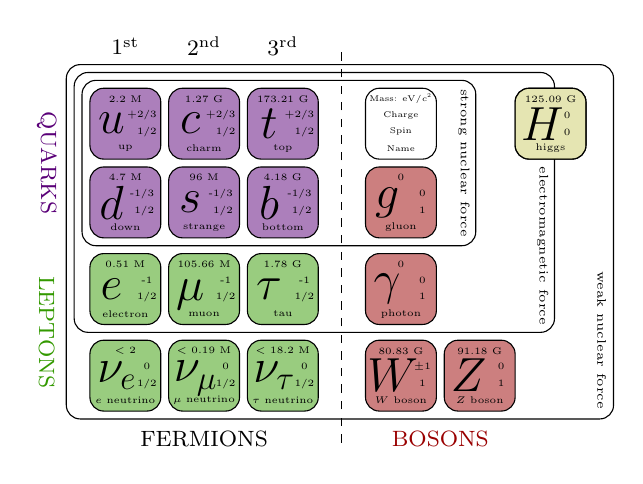
\begin{tikzpicture}[scale=1]

% frame
\draw[rounded corners=5,fill opacity=0] (-0.2,0.2) rectangle (6.75,-4-0.3);
\draw[rounded corners=5,fill opacity=0] (-0.1,0.1) rectangle (6,-3-0.2);
\draw[rounded corners=5,fill opacity=0] (-0.0,0.0) rectangle (5,-2-0.1);

% magenta squares
\draw[rounded corners=5,fill=cquarks,fill opacity=0.5] (0.1,-0.1) rectangle (1,-1) node[pos=0.5,opacity=1,xshift=-5,yshift=0] {\LARGE $u$} \leg{2.2 M}{+2/3}{\phantom{+}1/2}{up} node[pos=0.5,opacity=1,yshift=28] {\scalefont{0.8}$1^\mathrm{st}$};
\draw[rounded corners=5,fill=cquarks,fill opacity=0.5] (1+0.1,-0.1) rectangle (1+1,-1)node[pos=0.5,opacity=1,xshift=-5,yshift=0] {\LARGE $c$} \leg{1.27 G}{+2/3}{\phantom{+}1/2}{charm} node[pos=0.5,opacity=1,yshift=28] {\scalefont{0.8}$2^\mathrm{nd}$};
\draw[rounded corners=5,fill=cquarks,fill opacity=0.5] (2+0.1,-0.1) rectangle (2+1,-1)node[pos=0.5,opacity=1,xshift=-5] {\LARGE $t$} \leg{173.21 G}{+2/3}{\phantom{+}1/2}{top} node[pos=0.5,opacity=1,yshift=28] {\scalefont{0.8}$3^\mathrm{rd}$};
\draw[rounded corners=5,fill=cquarks,fill opacity=0.5] (0.1,-0.1-1) rectangle (1,-1-1)node[pos=0.5,opacity=1,xshift=-5] {\LARGE $d$} \leg{4.7 M}{-1/3}{\phantom{-}1/2}{down};
\draw[rounded corners=5,fill=cquarks,fill opacity=0.5] (1+0.1,-0.1-1) rectangle (1+1,-1-1)node[pos=0.5,opacity=1,xshift=-5,yshift=0] {\LARGE $s$} \leg{96 M}{-1/3}{\phantom{-}1/2}{strange};
\draw[rounded corners=5,fill=cquarks,fill opacity=0.5] (2+0.1,-0.1-1) rectangle (2+1,-1-1)node[pos=0.5,opacity=1,xshift=-5] {\LARGE $b$} \leg{4.18 G}{-1/3}{\phantom{-}1/2}{bottom};

% green squares
\draw[rounded corners=5,fill=clepts,fill opacity=0.5] (0.1,-0.2-2) rectangle (1,-1-2-0.1) node[pos=0.5,opacity=1,xshift=-5,yshift=0] {\LARGE $e$} \leg{0.51 M}{\phantom{+}-1}{\phantom{+}1/2}{electron};
\draw[rounded corners=5,fill=clepts,fill opacity=0.5] (1+0.1,-0.2-2) rectangle (1+1,-1-2-0.1) node[pos=0.5,opacity=1,xshift=-5,yshift=-2] {\LARGE $\mu$} \leg{105.66 M}{\phantom{+}-1}{\phantom{+}1/2}{muon};
\draw[rounded corners=5,fill=clepts,fill opacity=0.5] (2+0.1,-0.2-2) rectangle (2+1,-1-2-0.1) node[pos=0.5,opacity=1,xshift=-5,yshift=0] {\LARGE $\tau$} \leg{1.78 G}{\phantom{+}-1}{\phantom{+}1/2}{tau};
\draw[rounded corners=5,fill=clepts,fill opacity=0.5] (0.1,-0.3-3) rectangle (1,-1-3-0.2) node[pos=0.5,opacity=1,xshift=-3,yshift=0] {\LARGE $\nu_e$} \leg{< 2}{\phantom{+}0}{\phantom{+}1/2}{$e$ neutrino};
\draw[rounded corners=5,fill=clepts,fill opacity=0.5] (1+0.1,-0.3-3) rectangle (1+1,-1-3-0.2) node[pos=0.5,opacity=1,xshift=-3,yshift=-1] {\LARGE $\nu_\mu$} \leg{< 0.19 M}{\phantom{+}0}{\phantom{+}1/2}{$\mu$ neutrino};
\draw[rounded corners=5,fill=clepts,fill opacity=0.5] (2+0.1,-0.3-3) rectangle (2+1,-1-3-0.2) node[pos=0.5,opacity=1,xshift=-3,yshift=0] {\LARGE $\nu_\tau$} \leg{< 18.2 M}{\phantom{+}0}{\phantom{+}1/2}{$\tau$ neutrino};

% other squares
\draw[rounded corners=5,fill opacity=0] (3.5 + 0.1, -0.1) rectangle (3.5 + 1, -1)  \legInit;
\draw[rounded corners=5,fill=cbosons,fill opacity=0.5] (3.5 + 0.1, -1 - 0.1) rectangle (3.5 + 1, -2) node[pos=0.5,opacity=1,xshift=-5,yshift=0] {\LARGE $g$} \leg{0}{\phantom{+}0}{\phantom{+}1}{gluon};
\draw[rounded corners=5,fill=cbosons,fill opacity=0.5] (3.5 + 0.1, -2 - 0.2) rectangle (3.5 + 1, -3 - 0.1) node[pos=0.5,opacity=1,xshift=-5,yshift=0] {\LARGE $\gamma$} \leg{0}{\phantom{+}0}{\phantom{+}1}{photon};
\draw[rounded corners=5,fill=cbosons,fill opacity=0.5] (3.5 + 0.1, -3 - 0.3) rectangle (3.5 + 1, -4 - 0.2) node[pos=0.5,opacity=1,xshift=-3,yshift=0] {\LARGE $W$} \leg{80.83 G}{\phantom{+}$\pm1$}{\phantom{+}1}{$W$ boson};
\draw[rounded corners=5,fill=cbosons,fill opacity=0.5] (3.5 + 1 + 0.1, -3 - 0.3) rectangle (3.5 + 2, -4 - 0.2) node[pos=0.5,opacity=1,xshift=-4,yshift=0] {\LARGE $Z$} \leg{91.18 G}{\phantom{+}0}{\phantom{+}1}{$Z$ boson};
\draw[rounded corners=5,fill=white,fill opacity=1] (4.9 + 1 + 0.1-0.5, -0.1) rectangle (4.9 + 2-0.5, -1);
\draw[rounded corners=5,fill=paleale,fill opacity=0.5] (4.9 + 1 + 0.1-0.5, -0.1) rectangle (4.9 + 2-0.5, -1) node[pos=0.5,opacity=1,xshift=-3,yshift=0] {\LARGE $H$} \leg{125.09 G}{0}{0}{higgs};


% other stuff
\node[rotate=-90] at (5-0.15,-1.05) {\scalefont{0.45}strong nuclear force};
\node[rotate=-90] at (6-0.15,-2.1) {\scalefont{0.45}electromagnetic force};
\node[rotate=-90] at (7-0.15-0.25,-3.3) {\scalefont{0.45}weak nuclear force};

\node[color=cquarks,rotate=-90] at (-0.45,-1.05) {\scalefont{0.8}QUARKS};
\node[color=clepts,rotate=-90] at (-0.45,-3.2) {\scalefont{0.8}LEPTONS};
\node[color=black] at (1.55,-4-0.55) {\scalefont{0.8}FERMIONS};
\node[color=cbosons] at (4.55,-4-0.55) {\scalefont{0.8}BOSONS};

\draw[dashed] (3.3,-4-0.6) -- (3.3,0.45) ;

\end{tikzpicture}
\end{document}